\documentclass{beamer}
\usepackage[utf8]{inputenc}
\usetheme{Warsaw}

\usepackage{tikz,tkz-tab}

\newtheorem{proposition}{Proposition}
\newtheorem{exemple}{Exemple}

\title{Second degré.}
%\author{B. Meuhr}\institute{École Normale Supérieure, département de pipologie}

\begin{document}
  
  \begin{frame}
    
    \titlepage
    
  \end{frame}
  
  \section{Rappels de la classe de seconde.}
    
  \subsection{Variations de fonctions.}
  \begin{frame} %variations
    
    
    
    \begin{definition} 
      Une fonction est \textbf{croissante} (respectivement \textbf{décroissante}) sur un
      intervalle si les images de nombres dans cet intervalle sont rangées dans le même
      ordre (respectivement l'ordre inverse) que ces nombres.
    \end{definition}
    
    \uncover<2>
    {
      \begin{exemple}
      La fonction carré $\mathbb{R} \to \mathbb{R}, x \mapsto x^2$ est décroissante sur $]-\infty;0]$. 
      Par exemple, $(-2)^2=4>1=(-1)^2$. Pour exhiber les variations d'une fonction, 
      on construit souvent un tableau.
      \begin{center}
	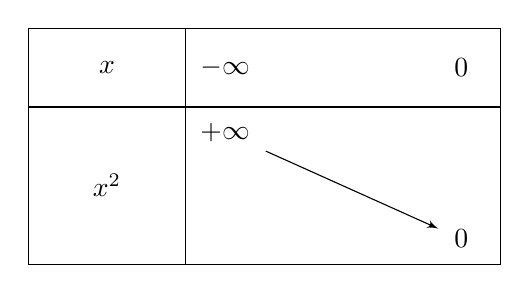
\begin{tikzpicture}
	  \tkzTabInit{$x$/1,$x^2$/2}{$-\infty$, $0$}
	  \tkzTabVar{+/$+\infty$,-/$0$}
	\end{tikzpicture} 
      \end{center}
      
    \end{exemple}
    }
  \end{frame}
  


  
  \begin{frame} %extremum    
    \begin{definition}
      
    Le \textbf{minimum} (respectivement le \textbf{maximum}) d’une fonction est la plus 
    petite (respectivement la plus grande) valeur atteinte par cette fonction.
    %Autrement dit, $m$ est le \textbf{minimum} (respectivement le \textbf{maximum}) de 
    %la fonction $f:E \to \R$ s'il existe $x_0$ dans $E$ tel que pour tout x 
    %dans $E$, ${m \leq f(x)}$ (respectivement $m \geq f(x)$).
    
    On appelle \textbf{extremum}, un minimum ou un maximum.
    \end{definition}
    
    \uncover<2,3,4,5,6>
    {
    \begin{exemple}
    D'après le tableau de variations précédent, 
    la fonction $f:]-\infty ; 0] \to \mathbb{R}, x \mapsto x^2$ 
    \uncover<3,4,5,6>{possède un minimum}
    \uncover<4,5,6>{, égal à $0$}
    \uncover<5,6>{, atteint pour $x=0$.}
    \uncover<6>{Mais $f(x)$ n'admet pas de maximum.}
    \end{exemple}
    }
  \end{frame}
  
  \subsection{Trinôme du second degré.}
  
  \begin{frame}
    \begin{definition}
      On dit qu'une fonction $f(x)$ est un trinôme du second degré si elle peut se mettre
      sous la forme $f(x)=ax^2+bx+c$ où $a$ doit être non nul.
    \end{definition}
    
    \begin{exemple}
      \begin{itemize}
      \item La fonction $g(x)=2x^2+3x+1$
      \uncover<2,3,4,5,6,7,8,9,10,11,12,13,14,15,16>{est un trinôme du second degré.}
      \item
      \uncover<3,4,5,6,7,8,9,10,11,12,13,14,15,16>{ La fonction $h(x)=3(x-1)^2+1$}
      \uncover<4,5,6,7,8,9,10,11,12,13,14,15,16>{est un trinôme du second degré.}
      \uncover<5,6,7,8,9,10,11,12,13,14,15,16>{En effet, $h(x)=$}
      \uncover<6,7,8,9,10,11,12,13,14,15,16>{$3(x^2-2x+1)+1=$}
      \uncover<7,8,9,10,11,12,13,14,15,16>{$3x^2-6x+4$.}
      \item 
      \uncover<8,9,10,11,12,13,14,15,16>{La fonction $i(x)=4(x-1)(x+2)$}
      \uncover<9,10,11,12,13,14,15,16>{est un trinôme du second degré.}
      \uncover<10,11,12,13,14,15,16>{En effet, $i(x)=$}
      \uncover<11,12,13,14,15,16>{$4(x^2-x+2x-1)=$}
      \uncover<12,13,14,15,16>{$4x^2+4x-4$.}
      \item 
      \uncover<13,14,15,16>{La fonction affine $i(x)=5x+3$}
      \uncover<14,15,16>{n'est pas un trinôme du second degré.}
      \item 
      \uncover<15,16>{Le polynôme $j(x)=x^3+4x^2+1$}
      \uncover<16>{n'est pas un trinôme du second degré.}
    
 \end{itemize}
     
 \end{exemple}
  \end{frame}  

  \subsection{Variations d'un trinôme du second degré}
  
  \begin{frame}
    \begin{theorem}
    Un polynôme de degré 2, $f(x)=ax^2+bx+c$ admet pour variations:
    
    \begin{center}
     
    
    \resizebox{11cm}{!}
    {
      \begin{tabular}{c c}
      Si $a>0$	
       
      
      &
       Si $a<0$
      
      
      \\
      
      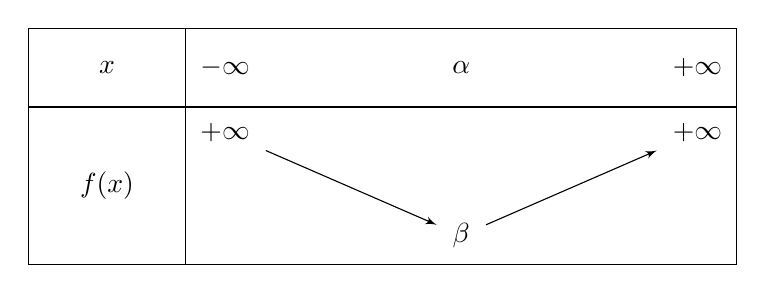
\begin{tikzpicture}
	\tkzTabInit{$x$ /1,$f(x)$/2}{$-\infty$, $\alpha$, $+\infty$}
	
	\tkzTabVar{+/$+\infty$,-/$\beta$,+/$+\infty$}
      \end{tikzpicture}
      &
      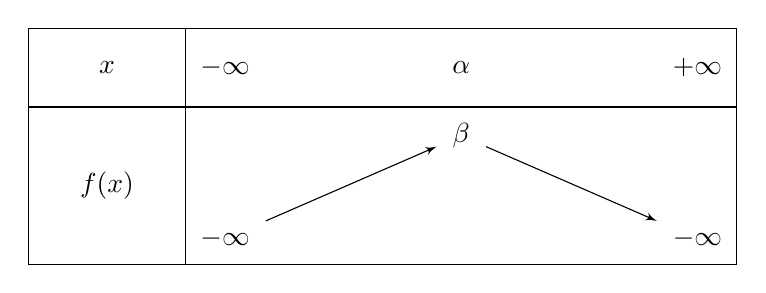
\begin{tikzpicture}
	\tkzTabInit{$x$/1,$f(x)$/2}{$-\infty$, $\alpha$, $+\infty$}
	
	\tkzTabVar{-/$-\infty$,+/$\beta$,-/$-\infty$}
      \end{tikzpicture}
      \end{tabular}
    }
    \end{center}
    
     On peut calculer les coordonnées $(\alpha,\beta)$ du sommet $S$ de la parabole grâce aux formules 
    $$\alpha=-\frac{b}{2a} \hspace{1cm} \beta=f(\alpha)$$
    
    \end{theorem}
  \end{frame}
  
    \section{Intersection d'une parabole avec l'axe des abscisses.}
    
    \begin{frame}
      
    \begin{proposition}[Positions de paraboles]
    Il n'y a que deux possibilités pour une parabole $\mathcal{P}:y=a(x-\alpha)^2+\beta$ 
    de couper l'axe des abscisses en deux points:
   \begin{itemize}
    \item Soit elle admet un minimum strictement négatif (cas $a>0, \beta <0$).
    \item Soit elle admet un maximum strictement positif.(cas $a<0\ et\ \beta >0$)
   \end{itemize}
   
   La parabole est tangente à l'axe des abscisses si et seulement si son extremum est 
   nul ($\beta=0$).

  \end{proposition}
   
  \end{frame}
	
     
      

      
      
      
      
    
    
   

  
\end{document}

\begin{itemize}
      
      
      
      
      
      
      
      
      

      
      
      
      
      
      
      
      
 \end{itemize}

  
  
  
  

\RequirePackage{framed} %  ou usepackage. permet d'encadrer les theo.

\RequirePackage[amsmath,thmmarks,hyperref,framed]{ntheorem}


\let\remarque\undefined

\theoremstyle{break}                  % passage à la ligne
\theorembodyfont{\itshape}     % fonte
\newtheorem{theoreme}{Th\'eor\`eme}
\newtheorem{proposition}{Proposition}
\newtheorem{propriete}{Propri\'et\'e}
\newtheorem{lemme}{Lemme}
\newtheorem{corollaire}{Corollaire}
\newtheorem{axiome}{Axiome}
\newframedtheorem{Theoreme}[theoreme]{Th\'eor\`eme} % theo. encadré
\newframedtheorem{Axiome}[axiome]{Axiome}
\newframedtheorem{Propriete}[propriete]{Propri\'et\'e}
%\newframedtheorem{Corollaire}[corollaire]{Corollaire}

\theorembodyfont{\upshape} % nouvelle fonte
\newtheorem{exemple}{Exemple}
\newtheorem{remarque}{Remarque}
\newtheorem{definition}{D\'efinition}
\newtheorem{convention}{Convention}
\newtheorem{note}{Note}
\newtheorem{representation}{Repr\'esentation graphique}
\newframedtheorem{Exemple}[exemple]{Exemple}


\theoremstyle{nonumberbreak} % pas de numerotation (de mémoire...)
\theoremheaderfont{\scshape}
\theoremsymbol{\ensuremath\square} % symbole en fin de theo.
\newtheorem{demonstration}{D\'emonstration}
\newtheorem{preuve}{D\'emonstration}